\section{Methods}
\label{sec:methods}

\subsection{Spiking network simulation}
\label{sub:methods_simulation}
Following Nordlie et al.'s suggestions on 
\emph{good model description practice} \cite{nordlie2009},
the network model is described in detail in the following paragraphs while a detailed 
overview is provided in two tables: The model is summarized in Table 
\ref{tab:model_description}, 
whereas specific numerical values of the parameters are displayed in Table 
\ref{tab:network_params}. 

\subsubsection{Model composition and connectivity}
% Model description
\begin{table}[htpb]
    \centering
    \caption{
        Model description according to Nordlie et al. \cite{nordlie2009}. 
        Specific parameters are shown in table \ref{tab:network_params}.
        }
    \label{tab:model_description}
    \begin{tabular}{m{3.1cm} p{10cm}}
        \rowcolor{TableColor}\multicolumn{2}{l}{Model summary} \\
        Populations     &   8 cortical populations\\
        Topology        &   --\\
        Connectivity    &   Random connections with fixed number of synapses for 
                            each combination of pre- and postsynaptic population\\
        Neuron model    &   Leaky integrate-and-fire, fixed voltage threshold, fixed 
                            absolute refractory period\\
        Synapse model   &   exponential-shaped postsynaptic current\\
        Plasticity      &   --\\
        Input           &   Independent fixed-rate Poisson spike trains\\
        Measurements    &   Spike activity, membrane potentials \tnn

        \rowcolor{TableColor} Populations & \\
        Layers          &   L23, L4, L5, L6 \\
        Cortical network&   one excitatory (e) and one inhibitory (i) population per layer\\
        Size            &   population specific size 
                            (see Table \ref{tab:network_params}) \tnn

        \rowcolor{TableColor} Connectivity & \\
        Type            &   Random connectivity with independently chosen pre- and postsynaptic
                            neurons; fixed total number of connections between two populations
                            (see Table \ref{tab:network_params}) \\
        Weights         &   Fixed; drawn from clipped Gaussian distributions 
                            ($w > 0$ for excitatory, $w~<~0$ for inhibitory)\\
        Delays          &   Fixed; drawn from clipped Gaussian distributions ($d~>~0$);
                            multiples of computation step size \tnn

        \rowcolor{TableColor}\multicolumn{2}{l}{ Neuron and synapse model} \\
        Name            &   iaf neuron\\
        Type            &   Leaky integrate-and-fire, exponential-shaped current inputs\\
        Subthreshold dynamics of neuron~$i$
                        &   {$\!\begin{aligned} 
                                \tau_\text{m} \,\dot{V_i}(t) 
                                    &= -(V_i(t) - E_\text{L}) + \frac{\tau_\text{m}}{C_\text{m}} I_i(t)
                                        &\text{if}\quad& t > t^* + \tau_\text{rp} \\ 
                                V_i(t)        
                                    &= V_\text{r}  &\text{else}& \\[0.2cm]
                                I_{\text{syn}, ij}(t) 
                                    &= w_{ij} \exp{\left(\frac{-t}{\tau_\text{syn}}\right)} \\[0.2cm]
                            \end{aligned}$}  \\
        Spiking         &   If $\,\,V_i(t_-) < \theta \quad \land \quad V_i(t_+) \ge \theta$: \\
                        &   \quad 1. set $t^* = t$    \\
                        &   \quad 2. emit spike with time stamp $t^*$ \tnn

        \rowcolor{TableColor} Input & \\
        Type            &   Independent Poisson spikes to iaf neurons
                            (see table \ref{tab:network_params})
    \end{tabular}
\end{table}

The network consists of eight cortical populations arranged in four 
layers. Each layer contains an excitatory as well as an inhibitory population.
A simplified diagram of the network is given in Figure \ref{fig:diagram}. 

\begin{figure}[htpb]
    \centering
    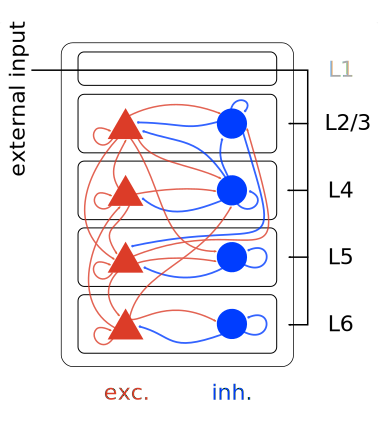
\includegraphics[width=0.5\linewidth]{../figures/diagram}
    \caption{Diagram of the layered cortical network. The displayed connections are only exemplary. 
    The external input is simulated by poissonian spike trains.}
    \label{fig:diagram}
\end{figure}

A total of 77169 leaky integrate-and-fire neurons are distributed according to the population
sizes given in Table \ref{tab:network_params}. The total numbers of excitatory and inhibitory 
neurons are 61843 and 15326, respectively, yielding a ratio of 4.04 of excitatory over inhibitory
neurons. \\
For each combination of pre- and postsynaptic population, pairs of neurons to be connected are drawn
randomly until a fixed number of synapses for each postsynaptic population is reached, 
allowing for multiple synapses and self-connections. 
Potjans' original model defines the connection probability $P_{\text{conn}, \,ab}$ 
of one neuron in the presynaptic population $a$ to form at least one connection with one neuron in 
the postsynaptic population $b$. For given population sizes $N_a$ and $N_b$, the number of 
synapses $C_{ab}$ is then calculated by
\begin{equation}
    C_{ab} = \frac{\ln \left( 1 - P_{\text{conn}, \,ab} \right)}{\ln \left( 1 - \frac{1}{N_a N_b} \right)} \, ,
    \label{eq:synapse_numbers}
\end{equation}
the inverse of the formula for connection probabilities derived by Potjans et. al \cite{potjans2014}.

The weight $w$ for each synapse is drawn from a normal distribution.
For excitatory presynaptic neurons, this mean value is set to $87,8$ pA (see below for 
a derivation). The mean for inhibitory ones is determined by multiplying 
with a factor $-g$, where the relative inhibitory synapse strength is set to 
$g = 4$. There is one important exception to this scheme.
The mean for the connection from L4e to L23e is increased by a factor of 
$j_{02} = 2$ (consult the corresponding paper \cite{potjans2014} for details). 
The standard deviation is set to $10\%$ of the mean. 
The distributions from which weights are drawn are clipped, 
such that a neuron assigned to the excitatory 
population will not have associated outgoing synapses with $w < 0$ 
and vice versa for inhibitory ones. 

Delays are drawn from normal distributions as well, with a mean value 
of $1.5$ ms for excitatory presynaptic neurons and half this value for 
inhibitory ones. The relative standard deviation is set to $0.5$. The distributions
are again clipped such that $d \ge 0$

\subsubsection{Neuron and synapse model}
The neurons are leaky integrate-and-fire neurons with a fixed voltage threshold. 
Below the threshold $\theta$, the dynamics of the membrane potential $V_i(t)$ 
for neuron $i$ are governed by the differential equation 
\begin{equation}
    \tau_\text{m} \,\frac{\text{d} V_i(t)}{\text{d} t} 
            = -(V_i(t) - E_\text{L}) + \frac{\tau_\text{m}}{C_\text{m}} I_i(t) \, .
    \label{eq:leaky_integrator}
\end{equation}
The membrane is specified by its resting potential $E_\text{L}$, 
its time constant $\tau_\text{m}$ and the capacitance $C_\text{m}$.
If, at time $t$, the threshold is reached, the neuron emits a spike and remains 
in a refractory period for a fixed time $\tau_\text{rp}$, with the membrane 
potential set to $V_\text{r}$. The total input to the neuron is represented by 
the current $I_i(t)$. 

The model implements  
postsynaptic current synapses with exponential shape, such that each 
spike arriving at one neuron leads to a current 
\begin{equation}
I_{\text{syn}}(t) = w \exp{\left(\frac{-t}{\tau_\text{syn}}\right)}	
    \label{eq:synaptic_current}
\end{equation}
where $w$ is the weight of the synapse in the model, given in pA
and $\tau_\text{syn}$ is the synapse time constant.
$w$ is identical to the amplitude of the postsynaptic 
current (PSC) at the time the spike arrives. 
Since measuring currents remains a difficult task for experimentalists, 
the model relays on measurements of the amplitude of the postsynaptic 
potential (PSP). In order to use the experimental observations, 
an approximative transformation is implemented 
by calculating the PSC induced if one spike with given PSP arrives at 
a neuron with membrane potential at rest. 
For $E_\text{L} = 0$, setting $I(t) = I_\text{syn}(t)$ in equation \eqref{eq:leaky_integrator}
yields:
\begin{equation}
    \dot{V}(t)
    = - \frac{1}{\tau_\text{m}} V(t) + \frac{w}{C_m} \exp{\left(-\frac{t}{\tau_\text{syn}}\right)} \,.
    \label{eq:psc_ode}
\end{equation}
This has the solution 
\begin{equation}
    V(t) =   
        - \frac{w \tau_\text{m} \tau_\text{syn}} {C_\text{m} \left(\tau_\text{m} - \tau_\text{syn}\right)}	
        \exp{\left( -\frac{t}{\tau_\text{syn}} \right)} 
        + C_1 \exp{\left(-\frac{t}{\tau_\text{m}} \right)}
    \label{eq:psc_ode_sol}
\end{equation}
with integration constant $C_1$.
With the boundary condition $V(t = 0) = 0$, this constant is set to
\begin{equation}
    C_1 = \frac{w \tau_\text{m} \tau_\text{syn}}{C_\text{m} \Delta\tau}	
    \label{eq:C_1}
\end{equation}
where $\Delta\tau := \tau_\text{m} - \tau_\text{syn}$ is introduced.
Thus
\begin{equation}
    V(t) = C_1 \left[\exp\left(-\frac{t}{\tau_\text{m}}\right) - \exp\left(-\frac{t}{\tau_\text{syn}}\right)\right]	\,.  
    \label{eq:V(t)}
\end{equation}

In order to get the PSP, we search for the maximum. Setting $\dot{V}(t) = 0$ 
yields
\begin{equation}
    t_\text{max} 
        = \ln{\!\left(\frac{\tau_\text{syn}}{\tau_\text{m}}\right)} 
            \left(\frac{1}{\tau_\text{m}} - \frac{1}{\tau_\text{syn}}\right)^{-1} \,.
    \label{eq:t_max}
\end{equation}
Inserting into equation \eqref{eq:V(t)} leads to 
\begin{equation}
    \text{PSP} := V(t_\text{max}) 
        = \frac{w \tau_\text{m} \tau_\text{syn}}{C_\text{m} \Delta\tau}	
            \left[ 
                \left( \frac{\tau_\text{syn}}{\tau_\text{m}} \right)^\frac{\tau_\text{syn}}{\Delta\tau} 
            - \left( \frac{\tau_\text{syn}}{\tau_\text{m}} \right)^\frac{\tau_\text{m}}{\Delta\tau} 
            \right]
    \label{eq:PSP}
\end{equation}
For a given PSP, this equation is simply inverted in order to get the according 
weight $w$. In this model, the PSP for excitatory neurons is set to 0.15 mV, 
which yields a PSC of 87.8 pA. 
Finally, the 
input current of neuron $i$ can be described as the sum over currents induced by
arriving spike trains, 
\begin{equation}
    I_i(t) = \sum_j w_{ij} \sum_k \exp\left(\frac{t - t_j^k - d_{ij}}{\tau_\text{syn}}\right) \, ,
    \label{eq:input_current}
\end{equation}
where $t_j^k$ is the time the $k$-th spike by neuron $j$ was emitted and the 
delay between neuron $i$ and $j$ is set to $d_{ij}$. 

\subsubsection{Model input, output and free parameters}
The model is solely driven by poissonian spike trains. Each neuron receives independent 
input at a rate specific to its population. This rate is determined by a global 
background rate of $8$ Hz multiplied by an external indegree $C_{a, \text{ext}}$ for
population $a$. This mimics a multiple number of synapses each transmitting the same input. 

The activity of the network is measured in terms of spike trains (measuring the spike times 
of single neurons up to the maximal simulation resolution $dt$) and membrane potentials in mV. 
The results in this thesis are based on recording only a fraction of the neurons in the network, 
choosing the first $n_a$ neurons of each population $a$. Since no topology is applied, this is 
equal to choosing $n_a$ neurons to record from randomly. If not specified else, spikes are recorded 
from $10\%$ of each population, membrane potentials from $2\%$. The further analysis of the data 
is explained in following sections.

The large number of free parameters of the model and their chosen values are summarized in 
Table \ref{tab:network_params}. 
% Network parameters
\begin{table}[htpb]
    \centering
    \caption{
        Network parameters
        }
    \label{tab:network_params}
    \begin{tabular}{p{3.5cm}| *{8}{x{1.2cm}}}
        \rowcolor{TableColor}\multicolumn{9}{l}{Populations and input} \tn 
        Name $a$       
            & L23e & L23i & L4e & L4i & L5e & L5i & L6e & L6i  \tn \hline
        Population size, $N_a$   
            & 20683 & 5834 & 21915 & 5479 & 4850 & 1065 & 14395 & 2948 \tn
        Ext. inputs, $C_{a, \text{ext}}$ 
            & 1600 & 1500 & 2100 & 1900 & 2000 & 1900 & 2900 & 2100 \tn[0.1cm]
        Background rate     
        &&&& 8 Hz \tnn

        \rowcolor{TableColor}\multicolumn{9}{l}{Connection probabilities between pre- and postsynaptic populations} \tn
        \diagbox[width=3.9cm]{post~~~~}{pre~~~}&
              L23e & L23i & L4e & L4i & L5e & L5i & L6e & L6i  \tn \hline
        L23e
            & 0.101 & 0.169 & 0.044 & 0.082 & 0.032 & 0.000 & 0.008 & 0.000 \tn 
        L23i
            & 0.135 & 0.137 & 0.032 & 0.051 & 0.075 & 0.000 & 0.004 & 0.000 \tn 
        L4e
            & 0.008 & 0.006 & 0.050 & 0.135 & 0.007 & 0.000 & 0.045 & 0.000 \tn 
        L4i
            & 0.069 & 0.003 & 0.079 & 0.160 & 0.003 & 0.000 & 0.106 & 0.000 \tn 
        L5e
            & 0.100 & 0.062 & 0.051 & 0.006 & 0.083 & 0.373 & 0.020 & 0.000 \tn 
        L5i
            & 0.055 & 0.027 & 0.026 & 0.002 & 0.060 & 0.316 & 0.009 & 0.000 \tn 
        L6e
            & 0.016 & 0.007 & 0.021 & 0.017 & 0.057 & 0.020 & 0.040 & 0.225 \tn 
        L6i
            & 0.036 & 0.001 & 0.003 & 0.001 & 0.028 & 0.008 & 0.066 & 0.144 \tnn

        \rowcolor{TableColor}\multicolumn{9}{l}{Further connectivity} \tn
        $w \pm \delta w$    
            &  \multicolumn{3}{l}{$87.8 \pm 8.8 \,\text{pA}$}
            &  \multicolumn{5}{l}{Excitatory synaptic strengths} \tn
        $j_{02}$    
            &  \multicolumn{3}{l}{$2$}
            &  \multicolumn{5}{l}{Factor for connection L4e $\to$ L23e} \tn
        $g$    
            &  \multicolumn{3}{l}{$4$}
            &  \multicolumn{5}{l}{Relative inhibitory synapse strength} \tn
        $d_e \pm \delta d_e$    
            &  \multicolumn{3}{l}{$1.5 \pm 0.75 \,\text{ms}$}
            &  \multicolumn{5}{l}{Excitatory synaptic transmission delays} \tn
        $d_i \pm \delta d_i$    
            &  \multicolumn{3}{l}{$0.8 \pm 0.4 \,\text{ms}$}
            &  \multicolumn{5}{l}{Inhibitory synaptic transmission delays} \tnn

        \rowcolor{TableColor}\multicolumn{9}{l}{Neuron model} \tn
        $\tau_\text{m}$    
            &  \multicolumn{3}{l}{$10 \,\text{ms}$}
            &  \multicolumn{5}{l}{Membrane time constant} \tn
        $\tau_\text{ref}$    
            &  \multicolumn{3}{l}{$\hphantom{0}2 \,\text{ms}$}
            &  \multicolumn{5}{l}{Absolute refractory period} \tn
        $\tau_\text{syn}$    
        &  \multicolumn{3}{l}{$\hphantom{0}0.5 \,\text{ms}$}
            &  \multicolumn{5}{l}{Postsynaptic current time constant} \tn
        $C_\text{m}$    
            &  \multicolumn{3}{l}{$250 \,\text{pF}$}
            &  \multicolumn{5}{l}{Membrane capacity} \tn
        $E_\text{L}$    
            &  \multicolumn{3}{l}{$-65 \,\text{mV}$}
            &  \multicolumn{5}{l}{Leaky rest potential} \tn
        $V_\text{reset}$    
            &  \multicolumn{3}{l}{$-65 \,\text{mV}$}
            &  \multicolumn{5}{l}{Reset potential} \tn
        $\theta$    
            &  \multicolumn{3}{l}{$-50 \,\text{mV}$}
            &  \multicolumn{5}{l}{Fixed firing threshold} \tn
    \end{tabular}
\end{table}

\subsubsection{Model validation}
some numbers and plots: 
single neuron response to poissonian input???
synapse numbers
number of autapses/repeated synapses
firing rates

\subsubsection{Model implementation}
Tools: pyNest, python, numpy/scipy, hdf5

include: version numbers

dt, exact integration?
number of kernels?

Put scripts online...

\subsection{Mean field model}
The derivation of a mean field theory goes along the 
lines of the work by Brunel \cite{brunel2000}.
It starts of with a simplified model of 
$N$ leaky integrate-and-fire neurons. 
Each neuron receives input from the network by $C$ synapses, 
$C_E$ from excitatory and $C_I$ from inhibitory ones. 
Furthermore, each neurons receives $C_\text{ext} = C_E$ connections from 
external excitatory neurons.
The synapse numbers 
are determined by the relative size of the two populations through the factor
\begin{equation}
    \epsilon := \frac{C_E}{N_E} = \frac{C_I}{N_I} \,.
    \label{eq:epsilon}
\end{equation}
A central assumption is the sparsity of the network, expressed by $\epsilon \ll 1$.
Guided by anatomical estimates for the neocortex, the population sizes are set to
$N_e = 0.8N$ excitatory and $N_i = 0.2N$ inhibitory neurons. Taking the definition
\eqref{eq:epsilon}, this implies 
\begin{equation}
    C_I = \gamma C_E 	
 \label{eq:C_I}
\end{equation}
with $\gamma = 0.25$. The synaptic weights in this model are set to $J$ for 
excitatory presynaptic neurons and to $-g\, J$ for inhibitory ones, 
whereas the delays are fixed uniformly to $d$ for all synapses. 

At the heart of the mean field model
is the transition from the deterministic description of membrane potential 
dynamics to a probabilistic formulation. 
As in Potjans' model, the membrane potential follows
the differential equation \eqref{eq:leaky_integrator}. The input is simplified 
by assuming an instantaneous and fixed change in membrane potential
for each spike arriving at the neuron instead of an exponential shaped PSC.
It can be described by a sum over Dirac delta-functions, 
\begin{equation}
    I_i(t) = \tau_\text{m} \sum_j J_{ij} \sum_k \delta(t - t_j^k - d_{ij}) \,.
    \label{eq:input_const_volt}
\end{equation}
The synaptic weights $J_{ij}$ in this case are equal to the PSP and given in mV.  

A number of conditions are necessary in order to make the transition from 
this description to a probabilistic one:
\begin{itemize}
    \item The sparsity implies that 
        two neurons share only a small number of common input such that pair correlations
        are negligible for $C / N \to 0$; 
    \item For the low single neuron firing rates $\nu$ compared to the 
        inverse membrane time constant $\tau_\text{a}$
        (e.~g. $\nu \sim10$ Hz and $1 / \tau_\text{m} \sim 1 / (20\,\text{ms}) = 50\, \text{Hz}$),
        a neuron receives a large number of small contributions per integration 
        time, each being very small compared to the threshold ($J \ll \theta$);
\end{itemize}
If these conditions are true, the input can be modeled as a time-varying average part
$\mu(t)$ plus a fluctuating gaussian part with amplitude $\sigma(t)$:
\begin{equation}
    \frac{\tau_\text{m}}{C_\text{m}} \, I_i(t) =  \mu(t) + \sigma(t) \sqrt{\tau_\text{m}} \eta_i(t) \, .
    \label{eq:input_random}
\end{equation}
The random fluctuations are described by gaussian white noise $\eta_i(t)$ with 
$\langle  \eta_i(t)\rangle = 0$. The model explicitly excludes correlations, 
both in time and between different neurons, i.e.
\begin{equation}
    \langle \eta_i(t) \: \eta_j(t') \rangle = \delta_{ij} \: \delta(t - t')	\, . 
    \label{eq:no_correlations}
\end{equation}
The latter assumptions has to be tested for the spiking model
that is to be described with this mean field approach. 

The fundamental parameter calculated by the mean field model is the single neuron
firing rate $\nu(t)$. In this basic model, it is assumed that any neuron of either 
of the two populations is firing with the same rate which is linked to the 
average input $\mu(t)$ by
\begin{equation}
    \begin{split}
        \mu(t)          &= \mu_l(t) + \mu_\text{ext} \\
        \text{with} \qquad \mu_l(t)        &= C_E \, J (1 - \gamma g) \nu(t - d) \tau_\text{m} \\
        \mu_\text{ext}  &= C_E J \nu_\text{ext} \tau_\text{m} \,.
        \label{eq:mu}
    \end{split}
\end{equation}
Similarly, for the amplitude of fluctuations $\sigma(t)$:
\begin{equation}
    \begin{split}
        \sigma^2(t)     &= {\sigma_l}^2(t) + {\sigma_\text{ext}}^2 \\
        \text{with} \qquad {\sigma_l}^2(t)       
                        &= C_E \, J^2 (1 + \gamma g^2) \nu(t - d) \tau_\text{m} \\
        {\sigma_\text{ext}}^2  &= C_E J^2 \nu_\text{ext} \tau_\text{m} \,.
        \label{eq:sigma}
    \end{split}
\end{equation}

Brunel then transforms equations \eqref{eq:input_random} and \eqref{eq:leaky_integrator}
into a Fokker-Planck equation describing the probability distribution of the membrane 
potential $P(V, t)$ in time: 
\begin{equation}
    \tau_\text{m} \, \frac{\partial P(V, t)}{\partial t} 
        = \frac{\sigma^2(t)}{2}  \: \frac{\partial^2 P(V, t)}{\partial V^2} 
         \quad + \quad \frac{\partial }{\partial V}  [(V- \mu(t)) P(V, t)] \, .
    \label{eq:fokker_planck}
\end{equation}
The probability distribution is subject to a number of 
constraints: Since the spiking resets neurons to $V_\text{rp} < \theta$, 
$P(V, t) = 0$ for $V > \theta$. Infinite probability currents are excluded 
such that $P(V, t)$ must be continuous at any point. Specifically, 
this continuity forbids infinity spiking probabilities at the threshold $\theta$. 
The resulting constraint is 
\begin{equation}
    P(\theta, t) = 0 \,.
    \label{eq:continuity} 
\end{equation}
Inserting this condition into equation \eqref{eq:fokker_planck} yields
\begin{equation}
    \frac{\partial P(\theta, t)}{\partial V}    
        = - \frac{2 \nu(t) \tau_\text{m}}{\sigma^2(t)}  \,.
\end{equation}
Neurons that fired at time $t$ come out of their refractory period at 
time $t + \tau_\text{rp}$ at the reset potential $V_\text{r}$. This leads to
a difference in probability current below and above $V_\text{r}$ proportional to 
the rate of neurons firing at $t - \tau_\text{rp}$ expressed by
\begin{equation}
    \frac{\partial P(V_r^+, t)}{\partial V} \: -  \: \frac{\partial P(V_r^-, t)}{\partial V} 
        = - \frac{2 \nu(t - \tau_\text{rp}) \tau_\text{m}}{\sigma^2(t)} \,.
\end{equation}
Finally, $P(V, t)$ is assumed to converge sufficiently quickly to zero:

\begin{equation}
    \lim_{V \to -\infty} P(V, t) = 0 
    \quad 
    \lim_{V \to -\infty} V P(V, t) = 0 \,.
\end{equation}

A stationary solution $P(V, t) = P_0(V)$ with constant 
single neuron firing rate $\nu_0$ 
satisfying the above boundary conditions is then presented:
\begin{equation}
    P_0(V) = 2 \frac{\nu_0 \tau_\text{m}}{\sigma_0} 
        \exp{\left(- \frac{(V - \mu_0)^2}{{\sigma_0}^2} \right)}
        \int_{\frac{V_r - \mu_0}{\sigma_0}}^{\frac{\theta - \mu_0}{\sigma_0}} \! 
            \Theta \left(u - \frac{V - \mu_0}{\sigma_0} \right) e^{u^2} \, \text{d}u  \,. 
    \label{eq:P_V_0}
\end{equation}
Here, $\Theta(x)$ is the Heaviside step function, i.~e. 
\begin{equation}
    \Theta(x) = \begin{cases} 1 & \text{if } x > 0 \\ 0 & \text{else } \end{cases}  \,.
    \label{eq:heaviside}
\end{equation}
The stationary mean input and fluctuation amplitudes are obtained by inserting 
$\nu_0$ into the equations \eqref{eq:mu} and \eqref{eq:sigma}, yielding 
\begin{align}
    \mu_0 	    &= C_E J \:\tau_\text{m} [\nu_\text{ext} + \nu_0(1 - g \gamma)]  \,, \\ 
    \sigma_0 	&= C_E J^{\,2} \,\tau_\text{m} [\nu_\text{ext} + \nu_0(1 + g^2 \gamma)] \,.
    \label{eq:mu_sigma_0}
\end{align}

In order to interpret $P(V, t)$ as a probability distribution, it is required to
satisfy the normalization condition
\begin{equation}
    \int_{-\infty}^{\theta} \! P(V, t) \, \text{d}V  + p_r(t) = 1 \, ,
    \label{eq:P_V_prob}
\end{equation}
where 
\begin{equation}
    p_r(t) := \int_{t - \tau_\text{rp}}^{t} \! \nu(u) \, \text{d}u 
    \label{eq:p_r}
\end{equation}
is the probability of neurons being the in refractory period.
In the constant case, this is simply 
\begin{equation}
    p_r(t) = p_{r, 0} = \nu_0 \tau_\text{rp}  \,.
    \label{eq:p_r_0}
\end{equation}

Inserting both $P_0(V)$ and $p_{r, 0}$ into the self-consistent condition \eqref{eq:P_V_prob}
then leads to an expression for $\nu_0$:
\begin{equation}
    \begin{split}
        \frac{1}{\nu_0} 	
            &= \tau_\text{rp} + \frac{1}{\nu_0} \int_{-\infty}^{\theta} \! P_0(V) \, \text{d}V  \\ 
            &= \tau_\text{rp} + \frac{2 \tau_\text{m}}{\sigma_0} 
                \int_{-\infty}^{\theta} \! \left[ 
                    \exp{\left(- \frac{(V - \mu_0)^2}{{\sigma_0}^2} \right)}
                    \int_{\frac{V_r - \mu_0}{\sigma_0}}^{\frac{\theta - \mu_0}{\sigma_0}} \! 
                        \Theta \left(u - \frac{V - \mu_0}{\sigma_0} \right) e^{u^2} \, \text{d}u 
                    \right] \, \text{d}V  \\ 
            &= \tau_\text{rp} + \frac{2 \tau_\text{m}}{\sigma_0} 
                \int_{\frac{V_r - \mu_0}{\sigma_0}}^{\frac{\theta - \mu_0}{\sigma_0}} \! 
                    \left[ 
                        e^{u^2}
                        \int_{-\infty}^{u \sigma_0 + \mu_0} \! 
                        \exp{\left(- \frac{(V - \mu_0)^2}{{\sigma_0}^2} \right)}
                        \, \text{d}V
                    \right] \, \text{d}u  \\ 
            &= \tau_\text{rp} + 2 \tau_\text{m}
                \int_{\frac{V_r - \mu_0}{\sigma_0}}^{\frac{\theta - \mu_0}{\sigma_0}} \! 
                    \left[ 
                        e^{u^2}
                        \int_{-\infty}^{u} \! e^{v^2} \, \text{d}v
                    \right] \, \text{d}u  \\ 
            &= \tau_\text{rp} + \tau_\text{m} \sqrt{\pi}
                \int_{\frac{V_r - \mu_0}{\sigma_0}}^{\frac{\theta - \mu_0}{\sigma_0}} \! 
                e^{u^2} \left(1 + \text{erf}(u)\right)
                \, \text{d}u  
        \label{eq:self_consistency}
    \end{split}
\end{equation}
This equation can be solved numerically for varying parameters as done by Brunel in order to 
characterize the different states the system can be found in. 

In order to transfer these results to the model of the neocortical microcircuit, 
the contributions to the input have to be adapted for each population. Instead of 
parametrized $\mu_0$ and $\sigma_0$ in terms of the variables $C_E$, $J$, $g$ and $\gamma$, 
a matrix notation as in equation \eqref{eq:synapse_numbers} is used: 
Synapse numbers and weights are defined as $C_{ab}$ and $J_{ab}$, respectively, 
where $a$ is the postsynaptic and $b$ the presynaptic population. 
Finally, the external input is written in a similar notation: 
An external excitatory population with single neuron firing rate $\nu_\text{ext}$ 
is connected to a neuron in population $a$ by 
$C_{a, \text{ext}}$ synapses of weight $J_{a, \text{ext}}$.
Including these definitions, the mean input and fluctuation amplitude can 
be written as 
\begin{align}
    \mu_a        &= 
        \tau_\text{m} \sum_{b \in \text{pop.}} C_{ab} \, J_{ab} \, \nu_b 
        + \tau_\text{m} C_{a, \text{ext}} \, J_{a, \text{ext}} \, \nu_\text{ext} \, ; \\
    {\sigma_a}^2 &= 
        \tau_\text{m} \sum_{b \in \text{pop.}} C_{ab} \, {J_{ab}}^2  \, \nu_b
        + \tau_\text{m} C_{a, \text{ext}} \,{J_{a, \text{ext}}}^2 \,\nu_\text{ext}\,,
\end{align}
where the sums go over all internal populations. In this specific case of eight 
populations one thus obtains eight equations for the 
firing rate $\nu_a$ of a single neuron in population $a$, 
\begin{equation}
    \frac{1}{\nu_{a}} = \tau_{rp} 
        + \tau_\text{m} \sqrt{\pi}
            \int_{\frac{V_r - \mu_{a}}{\sigma_{a}}}^{\frac{\theta - \mu_{a}}{\sigma_{a}}} 
                e^{u^2} \left(1 + \text{erf}(u)\right) \,\text{d}u  \,.
    \label{eq:self_consistency_a}
\end{equation}
These equations are coupled by the boundaries of the integrals. 



